\documentclass[12pt]{article}
\usepackage{graphicx}
\begin{document}
\begin{center}
{\large\bf The Sphericity Tensor and the Discovery of the Gluon}
\end{center}
\vskip0.2in
Goals:
\begin{itemize}
\item Learn how to calculate the sphericity tensor and understand how to interpret its eigenvalues
\item Reproduce, using simulated data, the analysis performed
  by Tasso to discover the gluon
\item Develop a simple event display as an aid to visualizing
  what two jet and three jet events look like in $e^+e^-$
  annihilation events
\end{itemize}
The first experimental evidence for the existence of the
gluon came from the analysis of data collected at the Petra
accelerator at DESY.  Several different analysis strategies
were used by the four collaborations (see
\begin{center}
  https://arxiv.org/pdf/1012.2288.pdf
\end{center}
for a review).  One such analysis, performed by the
Tasso group, was based on studies of the sphericity tensor:
$$
S_{\alpha\beta} = \frac{\sum_i p_{i\alpha} p_{i\beta}}{\sum_i
  \vec p_i^2}
$$
where the sum is over all charged particles in the event
(Tasso did not have good enough calorimetry to include neutrals
in the analysis) and the $\alpha$ and $\beta$ indices run
from 1 to 3, representing the $x$, $y$ and $z$ components
of the momentum vector.  For each event,
the Sphericity tensor can be
diagonalized to obtain the principle axes $\hat n_1$ through
$\hat n_3$ and eigenvalues $Q_1$ through $Q_3$.
With the definition of $S$ above, $Q_1+Q_2+Q_3=1$, so we only
need two eigenvalues to specify each event. 
If the
eigenvalues are ordered so that $Q_1<Q_2<Q_3$ then the
sphericity is defined to be
$$
S \equiv \frac{3}{2}\left (1 - Q_3\right )  = \frac{3}{2} \left (Q_1+Q_2 \right )
$$
and the aplanarity is defined to be
$$
A \equiv \frac{3}{2} Q_1 
$$
Here $0<S<1$ and $0<A < 0.5$.

Note that the form of the sphericity tensor is the same
as that of the moment of interia tensor (where the object's
position is replaced by its momentum).  We can therefore
use our intuition from classical mechanics to interpret this
tensor.  Long, thin rods have one large eigenvalue and two
small ones of rougly equal size, while a sphere has three
eigenvalues of equal size.  If we interpret the the
process $e^+e^-\rightarrow hadrons$ at parton level as
$e^+e^\rightarrow q\overline q$ we would expect most of
the momentum to flow along the original $q\overline q$ axis
with the momentum transverse to this direction limited by to
a scale set by $\Lambda_{QCD}$.  Thus, such events have $S$
close to zero.  The axis $n_3$ is a good estimate of
the initial direction of the back-to-back $q$ and $overline q$.
If instead,  a single hard gluon is radiated so that
the hard scattering process is $e^+e^\rightarrow q\overline qg$.
The events would appear planar with only a small component of 
momentum outside the plane.
Here is what Tasso observed:
\begin{figure}[h]
  \begin{center}
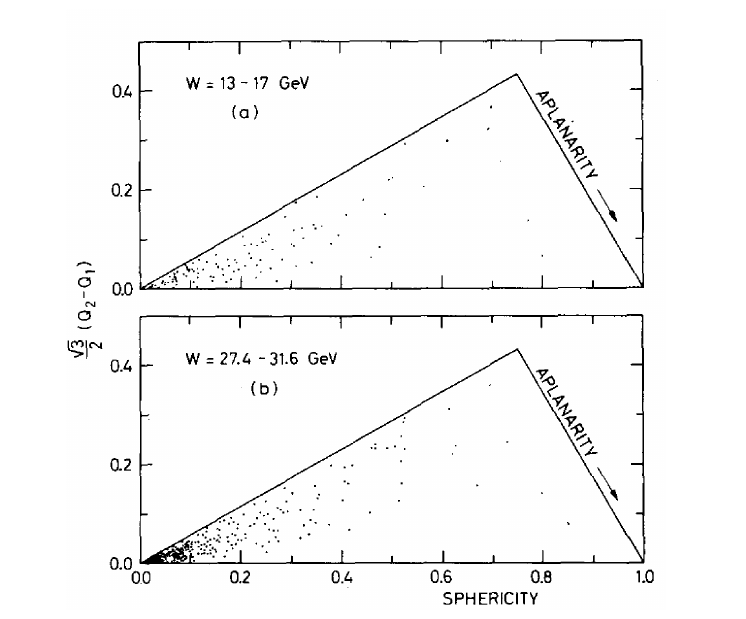
\includegraphics[width=3.8in]{tassoSphericityAplanarity.png}
  \end{center}
  {Distribution of the sphericity and aplanarity
    of $e^+e^-\rightarrow hadron$ events measured by
  the TASSO collaboration in R.
Brandelik et al., {\it Evidence for Planar Events in e+e− Annihilation at High Energies}, Phys. Lett. B 86, 243 (1979).}
\end{figure}

You will now reproduce their analysis using simulated
data created with the Pythia8 Monte Carlo generator.  The file
{\bf Pythia8e+e-Toqqbar36GeV.dat} contains the charged particle information
for 10000 events.  The format of the file is specified
in the metadata comments at the beginning of the file.
\begin{enumerate}
\item[(a)] For each event in the file, calculate the
  sphericity tensor and find its eigenvalues.  Plot the
  data using the same $x$ and $y$ axes as the Tasso plot
  above.
\item[(b)] As discussed above, the momentum along the $\hat n_3$
  axis should be larger than in the other directions.
  The momentum along the $\hat n_2$
  direction should be small for 2-jet events, with a tail
  extending to larger values of momentum for
  3-jet events where a gluon is radiated.  The momentum
  along the $\hat n_1$ direction should be small unless more
  than one gluon is radiated.  Since $\alpha_S\approx 0.12$ at Petra
  energies, the probability of
  multiple hard gluon radiation is small.  Make
  histograms of the components of momentum along each
  of the three principle axes for the events you have analyzed.
  What do these plots show?
\item[(c)] When physicists observe a new phenomenon, they often
  like to display individual events to make sure they ``look''
  they way we expect.  We can display a single event by
  making a 3D plot with a vector representing the momentum
  of each charged particle.  Make such four such displays,
  two for
  events with $S<0.05$ and two for events with $S>0.3$.  Do
  they look the way you expect them to?
\end{enumerate}
\end{document}
